\section{Ramp Rate Analysis} %4.5
\label{section4.5}

From Section~\ref{section3.5}, we understand the importance of using ramp rate in power system. The aim is to be realistic. This is a real constraint in physical systems. The control cannot be used in reality if do not set the limit of it.\\

In Section~\ref{section3.5}, we discussed the reason to use \sys{peak} and \sys{peaktime} to calculate the ramp rate. Equation is as follow.

\begin{equation}
    Rate = \frac{P_{\sys{peak}} - P_o}{\sys{PeakTime}}
\end{equation}


Next, we can calculate the limit of ramp rate of generators. According to National Renewable Energy Lab., Golden, CO (US), \cite{osti_15016292} large thermal units are usually able to ramp around 1\% of their capacity per minute. Thus, we have Table~\ref{4_5_nominal_rate}:


\begin{table}[htbp]
  \centering
    \begin{tabular}{ccccc}
    Generator & Pnom~\footnote{Pnom (nominal power) is original from:~\href{https://github.com/realgjl/sfcNordic/blob/master/examples/dyn\_A.dat}{https://github.com/realgjl/sfcNordic/blob/master/examples/dyn\_A.dat}} (MW) & Ramp Rate (MW/min) & Ramp Rate (MW/sec)\\
    g6    & 360   & 3.6   & 0.06\\
    g7    & 180   & 1.8   & 0.03\\
    g14   & 630   & 6.3   & 0.105\\
    g15   & 1080  & 10.8  & 0.18\\
    g16   & 630   & 6.3   & 0.105\\
    \end{tabular}
  \caption{Nominal ramp rate of generators}
  \label{4_5_nominal_rate}
\end{table}

Then we can use the limit of ramp rate from Table~\ref{4_5_nominal_rate} to remove some tuning results. The source code~\footnote{See \href{https://github.com/realgjl/sfcNordic/blob/master/analysis/4.5/risk\_lowTd.m}{https://github.com/realgjl/sfcNordic/blob/master/analysis/4.5/risk\_lowTd.m}} is open to public. \\

\begin{table*}[htbp]
\centering
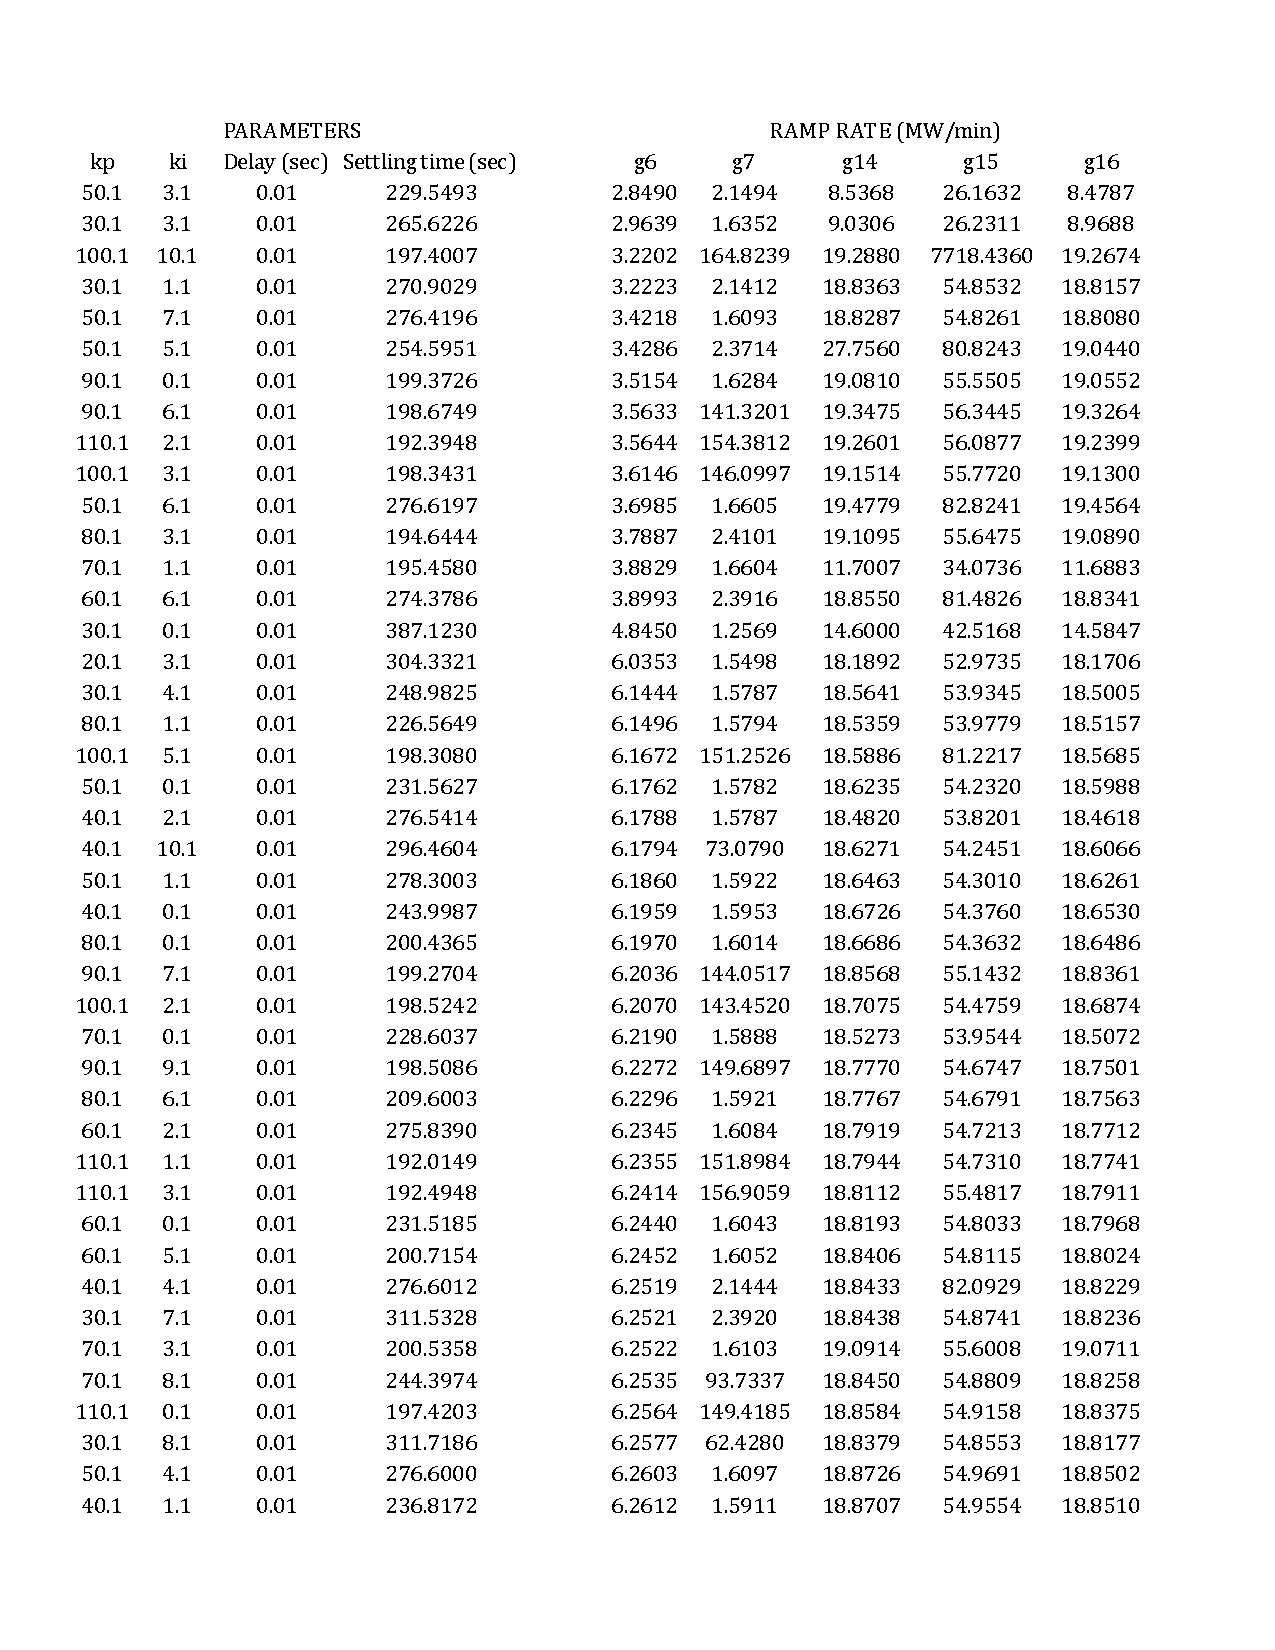
\includegraphics[width = \textwidth]{figure/4_5_risk.pdf}
\caption{Some generators' real ramp rates, ranked by g6's ramp rate.}
\label{4_5_risk}
\end{table*}


Finally, we should have a figure that similar to Figure~\ref{4_4_1_2d}. However, as you can see from Table~\ref{4_5_risk}, none of tuning results can meet the requirement of the limit of ramp rate (i.e. the ramp rates in the test system are larger than the limit). After repeated confirmation, I do not think there are any logic mistake in my algorithm. \\

In fact, our assumption is based on the materials from the United States. Although it's positive to reference an official document, the situation might be different between the United States and Nordic countries.\\

Wärtsilä Oyj Abp, a Finnish corporation which manufactures and services power sources and other equipment in the marine and energy markets, says, \cite{Combustion} "Ramp rates of most industrial frame gas turbine models are advertised as 10 MW/min up to 100 MW/min, with an average of about 25 MW/min". The maximum allowed ramp rate or the average one are significantly larger than the limit we set.\\

Another paper is also mentioned the similar information that, in Germany, \cite{huber2017flexibility} the maximum ramp can be up to 11\%.

Thus, it's reasonable to believe that, in Nordic grid, the official ramp rate should be larger than 1\% of the nominal power per min.\\


Another conclusion that we can sum up from Table~\ref{4_5_risk} is that storage ramp rates are rapid (i.e. output can change quite rapidly). Power devices with a slow response time tend to have a slow ramp rate. This is the philosophical inspiration of Smart Grid operation: a fast response time would exceed the physical limit of a turbine which forces you to slow the response time to keep a balance between the design and the requirement.\\